\chapter{线性模型}
\section{基本形式}
线性模型是统计学中一种重要的模型形式,通常用于描述因变量与一个或多个自变量之间的线性关系。其向量形式可以表示为:
\begin{equation}
\mathbf{y} = \beta^\top \mathbf{X} + \epsilon
\end{equation}
其中,$\mathbf{y}$ 是因变量的观测值向量,$\mathbf{X}$ 是自变量的设计矩阵,$\beta$ 是待估计的参数向量,$\epsilon$ 是误差项。
\section{线性回归}
最小二乘法是线性模型中最常用的参数估计方法,其目标是最小化观测值与模型预测值之间的平方差:
\begin{equation}
\hat{\beta} = \arg\min_{\beta} \|\mathbf{y} - \mathbf{X} \beta\|^2
\end{equation}
其中, $\hat{\beta}$ 是参数的估计值。$arg\min$ 表示取使目标函数最小化的参数值。

当$\mathbf{X}^\top \mathbf{X}$ 不是满秩时,最小二乘法的解可能不唯一,此时可以使用岭回归等方法进行正则化,以获得更稳定的参数估计。

广义线性模型(GLM)是线性模型的推广,允许因变量服从非正态分布,并通过链接函数将期望值与线性预测器联系起来。GLM的形式为:
\begin{equation}
    g(\mathbb{E}[Y|\mathbf{X}]) = \beta^\top \mathbf{X}
\end{equation}
其中,$g(\cdot)$ 是链接函数,$\mathbb{E}[Y|\mathbf{X}]$ 是因变量的条件期望。例如,当$g(\cdot)=\log(\cdot)$时,GLM为对数线性模型,适用于计数数据;当$g(\cdot)=\text{logit}(\cdot)$时,GLM为逻辑回归模型,适用于二分类数据。
\begin{lstlisting}[language=Matlab, caption=线性回归的Matlab代码,label=lst:linear_regression]
% 线性回归的Matlab代码示例
clc,clear;
% 生成模拟数据
n = 100; % 样本数量
X = [ones(n, 1), randn(n, 2)]; % 自变量矩阵,第一列为常数项(截距)
beta_true = [1; 2; 3]; % 真实参数
y = X * beta_true + randn(n, 1) * 0.5; % 添加噪声生成因变量

% 拟合线性回归模型
mdl = fitlm(X, y);

% 输出回归结果
disp('参数估计:');
disp(mdl.Coefficients.Estimate);
disp(['R方: ', num2str(mdl.Rsquared.Ordinary)]);
disp(['调整后的R方: ', num2str(mdl.Rsquared.Adjusted)]);
disp(['均方误差: ', num2str(mean(mdl.Residuals.Raw.^2))]);

% 绘制回归结果及诊断图
figure;
plot(mdl);
title('线性回归拟合图');

% 输出结果
%{
参数估计:
         0
    1.0325
    2.0137
    3.0050
R方: 0.98584
调整后的R方: 0.98555
均方误差: 0.22526
%}
\end{lstlisting}
\begin{figure}[H]
    \centering
    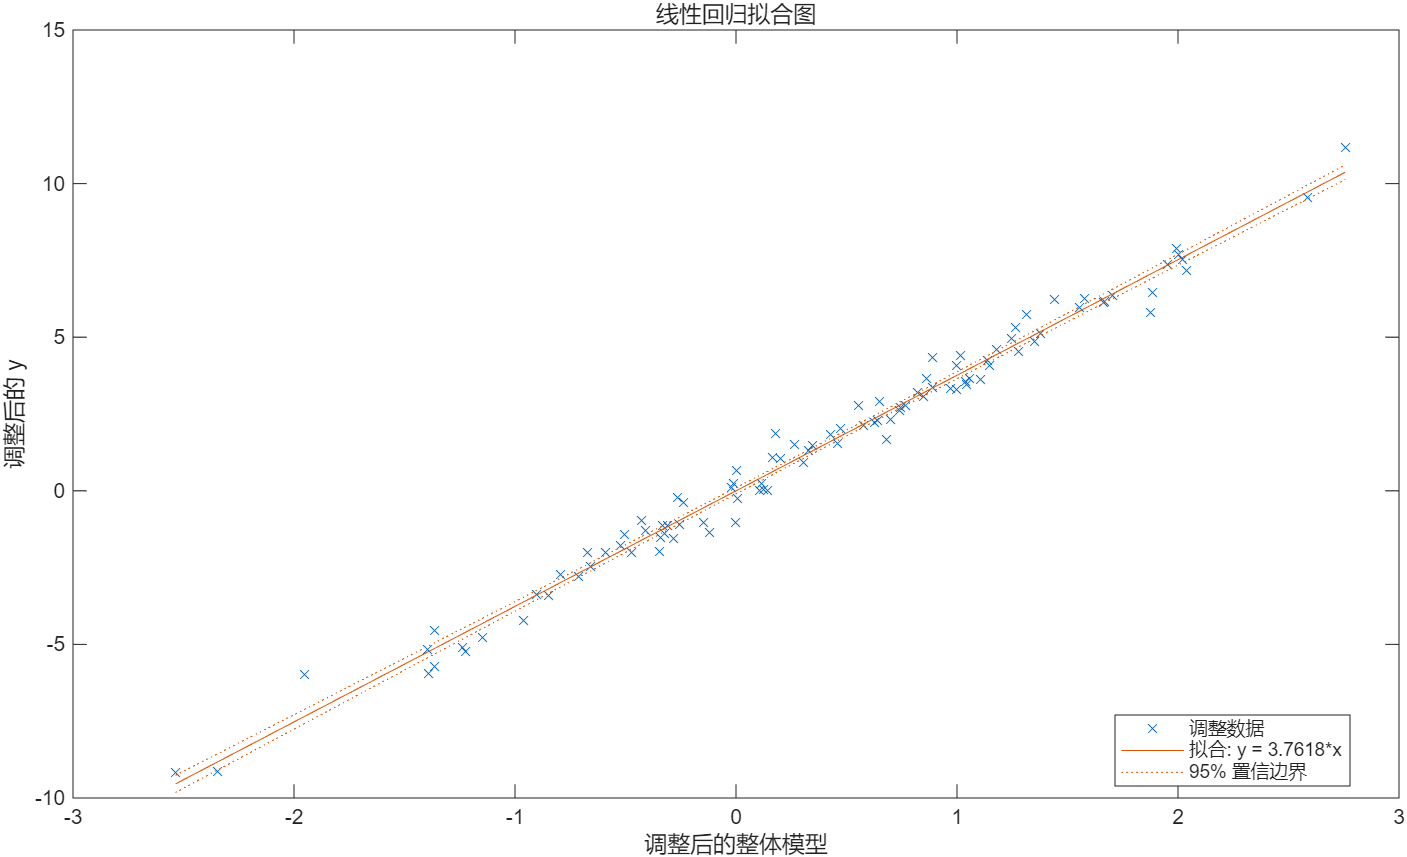
\includegraphics[width=0.8\textwidth]{./static/images/线性回归图.png}
    \caption{线性回归拟合结果}
    \label{fig:linear_regression_fit}
\end{figure}
\section{对数几率回归}
对数几率回归(Logistic Regression)是一种广义线性模型,主要用于二分类问题。其模型形式为:
\begin{equation}
    P(Y=1|\mathbf{X}) = g(\beta^\top \mathbf{X}) = \frac{1}{1 + e^{-\beta^\top \mathbf{X}}}
\end{equation}
其中,$P(Y=1|\mathbf{X})$ 是在给定自变量$\mathbf{X}$的条件下,因变量$Y$取值为1的概率,$g(\cdot)$ 是sigmoid函数。
